\chapter{相关理论技术研究}
点云是在同一空间参考系下目标物体的空间分布的大量点集合,点云图像是最基础也是最常见的三维图像。点云配准是将多个来自不同传感器或不同时间、空间的点云数据进行对齐和融合的过程。毫米波雷达的点云配准,是结合毫米波雷达自身数据特征,将多个毫米波雷达位于不同空间位置获取的点云进行融合。借助多个毫米波雷达配准后的点云获取更全面并且一致的环境信息。
\section{调频连续波雷达相关技术}
调频连续波雷达(Frequency Modulated Continuous Wave,FMCW)\cite{brooker2005understanding}是一种采用频率调制技术的雷达系统,主要用于测距和速度测量。相较于传统脉冲雷达,FMCW雷达在发送连续波形的同时进行频率调制,实现了对目标距离和速度的同时测量。 FMCW雷达主要由三个部分组成:发射部分、接收部分和处理部分。发射部分发射信号,经过物体反射由接收部分接收后经过混频器放大到中频,由处理部分获取目标的距离和速度信息。FMCW雷达的原理如图\ref{fmcw}所示。

\begin{figure}[htbp]
	\centering
	% Requires \usepackage{graphicx}
	\includegraphics[width=0.5\textwidth]{figures/fmcw.pdf}\\
	\caption{FMCW雷达框图}
	\label{fmcw}
\end{figure}

\subsection{FMCW雷达测距}
合成器生成的信号称为Chrip信号,Chrip信号频率随时间线性变化,信号时域图和频域图如图\ref{chrip},通常发射信号的频率在一个较小的范围内变化。每次发送与接收到的回波信号与发射信号之间存在频率差。接收部分中的混频器用于将接收到的信号与本地振荡器的信号混频产生中频(Intermediate Frequency,IF)信号\cite{waters1982bandpass}。中频信号随时间的变化包含了目标的距离和速度信息。

\begin{figure}[htbp]
	\centering
	% Requires \usepackage{graphicx}
	\includegraphics[width=0.8\linewidth]{figures/Chrip信号时频域图}\\
	\caption{Chrip信号时频域图}
	\label{chrip}
\end{figure}

FMCW雷达在$t_1$时刻合成器合成频率为$f_1$的Chrip信号,经过物体对该信号的反射,生成一个由接收天线捕捉的信号。在经过延时$\tau$后由接收天线收到信号,混频器将收到的信号与发送信号混合,生成一个具有新频率的新信号。如公式\eqref{signal1}和\eqref{signal2}表示两个输入的正弦信号$x_1$和$x_2$。
\begin{equation}
	x_1 = \sin(\omega_1t+\Phi_1)
	\label{signal1}
\end{equation}
\begin{equation}
	x_2 = \sin(\omega_2t+\Phi_2)
	\label{signal2}
\end{equation}
经过混频器混合后得到$x_3$。
\begin{equation}
	x_3 = \frac{1}{2}\sin \big(\left(\omega_1 + \omega_2\right)t + \Phi_1+ \Phi_2\big) + 
	\frac{1}{2}\sin \big(\left(\omega_1 - \omega_2\right)t + \Phi_1- \Phi_2\big) 
\end{equation}
经过低通滤波后,得到如公式\eqref{signal_out}所示的中频信号$x_{out}$,其频率为$x_1$与$x_2$频率的差值。
\begin{equation}
	x_{out} = \frac{1}{2} \sin\big((\omega_1 - \omega_2)t + \Phi_1- \Phi_2\big)
	\label{signal_out}
\end{equation}
混频器的运行方式如图\ref{IF}所示,图像中两条线的距离固定,表示 IF 信号包含一个频率恒定的信号,此信号为公式\eqref{signal_out}所代表信号,只存在于两个信号叠加的阶段。其频率是$\Delta f $。图\ref{IF}中信号变化的速率即图像的斜率$S$已知,因此可以使用公式\eqref{tau0}计算出延时$\tau$。
\begin{figure}[htbp]
	\centering
	% Requires \usepackage{graphicx}
	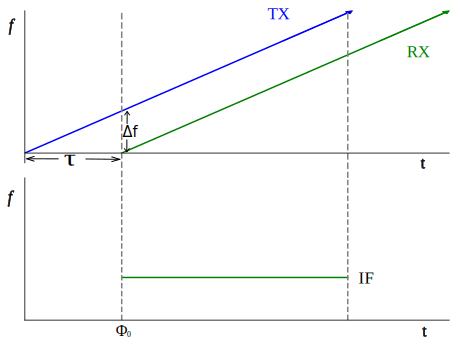
\includegraphics[width=0.6\textwidth]{figures/if1.pdf}\\
	\caption{IF 频率恒定不变}
	\label{IF}
\end{figure}

\begin{equation}
	\tau = \frac{\Delta f}{S}
	\label{tau0}
\end{equation}
通过公式\eqref{tau1}代入$\tau$后可推导出$d$,其中 $d$ 是与被检测物体的距离,$c$ 是光速。
\begin{equation}
	\tau = \frac{2d}{c}
	\label{tau1}
\end{equation}
图\ref{IF}中IF 信号的初始相位$\Phi_0$是IF信号起点对应的时间点,即图\ref{IF}中左侧垂直虚线表示的时间点发送信号相位与接收信号相位之差。
\begin{equation}
	\Phi_0 = 2\pi f_c \tau = \frac{4\pi d}{\lambda}
	\label{phi0}
\end{equation}

\begin{figure}[htbp]
	\centering
	% Requires \usepackage{graphicx}
	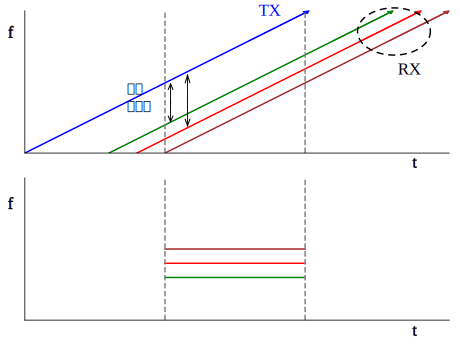
\includegraphics[width=0.6\textwidth]{figures/ifs.pdf}\\
	\caption{多个物体IF信号}
	\label{IFS}
\end{figure}


在检测多个物体的情况下会收到多个物体的反射信号。每个反射信号的延时都不一样,延时与该物体的距离成正比。不同的反射信号转化为多个IF中频信号并混合在一起如图\ref{IFS},每个信号频率恒定。这个包含多个信号的IF信号必须使用傅里叶变换加以处理,以便分离不同的IF中频信号。傅里叶变换处理将会产生一个具有不同的分离峰值的频谱,每个峰值代表对应的距离处存在物体。


\subsection{FMCW雷达测速}
为测量速度,FMCW雷达会周期性地发送Chrip信号,每个Chrip之间存在$T_c$的时间间隔。目标反射的信号通过距离维FFT检测目标的距离。对应于每个线性调频脉冲的距离维FFT将在同一位置出现峰值\cite{rao2017introduction},但相位不同。测得的相位差与速度为$v$的物体在$T_c$间隔的移动对应。相位差可以通过公式\eqref{phi0}推导出公式\eqref{deltaPhi}:
\begin{equation}
	\Delta \Phi = \frac{4\pi V_{T_c}}{\lambda}
	\label{deltaPhi}
\end{equation}
可以通过公式\eqref{v1}推导出速度:
\begin{equation}
	v = \frac{\lambda \Delta \Phi}{4\pi T_c}
	\label{v1}
\end{equation}
由于基于相位差的速度测量仅在$\lvert \Delta \Phi \rvert < \pi $时具有非模糊性\cite{atlas1973doppler},所以使用上述公式可以推断出测速的范围为:
\begin{equation}
	v< \frac{\lambda}{4T_c}
\end{equation}
因此更短的传输间隔可以测量更快的速度。

由离散傅里叶变换\cite{wang1984fast}可知,两个离散的频率$\omega_1$和$\omega_2$在$\omega_1 - \omega_2 > \frac{2\pi}{N}$(N为样本个数)的前提下才可以分辨。因此从公式\eqref{deltaPhi}可知:

\begin{equation}
	\frac{4\pi V_{T_c}}{\lambda} > \frac{2\pi}{N}
\end{equation}
代入帧周期$T_f = N T_c$可得:
\begin{equation}
	v > \frac{\lambda}{2N T_c} = \frac{\lambda}{2 T_f}
\end{equation}
雷达的速度分辨率与帧时间成反比。

% \subsection{CFAR算法} % todo CFAR算法

\section{点云配准相关技术}

\subsection{刚性点云配准算法}
刚性点云配准主要目标是找到两个点云之间的最佳转换\cite{tam2012registration},以使它们在空间中更好地对齐。刚性点云配准是一种在计算机视觉和机器人领域广泛应用的点云配准方法\cite{JSJX201909003}。其基本原理是通过迭代的方式,不断优化两个点云之间的刚体变换使它们的重叠部分最大化。

首先,通过某种方式初始化两个点云的初始对准。可以通过随机设置初始值、粗略的估计、传感器测量或其他方法实现。
通过计算每个点在参考点云中的最近邻点,建立点云之间的初始对应关系。这一步通常使用KD树\cite{bentley1990k}等数据结构来提高匹配效率,KD树的实现算伪代码如算法\ref{alg:kdtree}所示。

\begin{algorithm}[htbp]
	\caption{构建KD树}\label{alg:kdtree}
	\begin{algorithmic}[1]
		\Require 点集$X$,深度$depth$
		\Ensure KD树
		\If{$\text{点集}$ 为空}
		\State \textbf{return} $\text{NULL}$
		\EndIf
		\State $k \gets$ 点的维度
		\State $axis \gets depth \mod k$
		
		\State $P \gets \text{按轴排序}(X, axis)$ \Comment{沿着所选轴对点进行排序}
		
		\State $medianIndex  \gets \text{点集长度} \div 2$ \Comment{获取中值索引}
		
		\State $median \gets P[medianIndex]$ \Comment{获取中值}
		
		\State $node \gets \text{创建节点}(median, axis)$ \Comment{创建一个新的KD树节点}
		
		\State $node.left \gets \text{构建KD树}(P[1 : medianIndex-1], depth + 1)$
		\State $node.right \gets \text{构建KD树}(P[medianIndex+1 : len(P)], depth + 1)$
		
		\State \textbf{return} node
	\end{algorithmic}
\end{algorithm}

利用最近邻匹配得到的对应关系,计算两个点云之间的最佳刚体变换,通常采用最小二乘法等优化算法。在采用最小二乘法计算点云距离的算法中,通过拟合一个模型来估计点云之间的距离。最小二乘法的核心思想是最小化残差平方和,即观测值与模型预测值之间的差异。假设有源点云$P$和参考点云$Q$如公式\eqref{点云表示}所示,其中$P$和$Q$分别表示源点云和参考点云,$p_i$和$q_i$分别表示源点云和参考点云中的点。需要求出变换矩阵$R$和平移变量$t$使得$\forall i, q_i=Rp_i + t$。
\begin{equation}
	\label{点云表示}
	\begin{split}
		P =  \left\lbrace p_1, p_2,\ldots,p_n \right\rbrace\\
		Q =  \left\lbrace q_1, q_2,\ldots,q_n \right\rbrace
	\end{split}
\end{equation}

使用初始的$R_0,t_0$或上一次迭代得到的的$R_k,t_k$ 对初始点云进行变换,得到一个临时变换的点云,然后继续用得到的点云与参考点云进行比较,找出当前源点云中每一个点在参考点云中的最近邻点,基于最小二乘法进行迭代计算,使得误差平方和达到极小值。

\begin{equation}
\label{最小化Rt}
R,t = \mathop{\arg\min}_{R,t}\sum_{i=1}^{n} \|\left( Rp_i+t\right) -q_i \| ^2
\end{equation}


计算最优平移$t$,令 $N=|P|$ ,由公式\eqref{最小化Rt}可知,此时迭代的损失表示为:
\begin{equation}
	\label{损失公式1}
	F(t) = \sum_{i=1}^{N} \| (R\cdot p_i + t) - q_i\|^2
\end{equation}

对损失求偏导可得:
\begin{equation}
	\label{损失公式1偏导}
	\begin{split}
		\frac{\partial F}{\partial t} &= \sum_{i=1}^{N}2(R \cdot p_i + t-q_i)\\
		&=2nt + 2R\sum_{i=1}^{N}p_i -  2R\sum_{i=1}^{N}q_i
	\end{split}
\end{equation}


令$\frac{\partial F}{\partial t} = 0$,可得:
\begin{equation}
	\label{最优平移计算}
	\begin{split}
			t &= \frac{1}{N}\sum_{i=1}^{N} q_i - R\sum_{i=1}^{N}p_i\\
		&= \bar{q} - R\bar{x}
	\end{split}
\end{equation}

由公式\eqref{最优平移计算}可知,loss最小的最优平移可以由最优旋转$R$和两个点云的质心求出。

接下来求最优旋转$R$,由最佳平移的证明过程可知,最优平移由最优旋转通过点云的质心计算得到。为了计算简单,先将点云所有的点以质心为中心平移。即令$\hat{p_i} = p_i - \bar{p}$,$\hat{q_i} = q_i - \bar{q}$。此时loss的形式转变为:

\begin{equation}
	\label{损失公式}
	F(R) = \sum_{i=1}^{N} \| R\cdot\hat{p_i} - \hat{q_i}  \|^2
\end{equation}
先对$ \| R\cdot\hat{p_i} - \hat{q_i}  \|^2$ 进行公式\eqref{eq:绝对值计算}计算:
\begin{equation}
	\label{eq:绝对值计算}
	\begin{split}
		\| R\cdot\hat{p_i} - \hat{q_i}  \|^2 &= ( R\cdot\hat{p_i} - \hat{q_i})^T ( R\cdot\hat{p_i} - \hat{q_i}) \\
		&= ( \hat{p_i}^T \cdot R^T - \hat{q_i}^T) ( R\cdot\hat{p_i} - \hat{q_i}) \\
		&= \hat{p_i}^T \cdot R^T  R\cdot\hat{p_i} -  \hat{p_i}^T \cdot R^T  \hat{q_i} -  \hat{q_i}^TR\cdot\hat{p_i} +  \hat{p_i}^T \hat{q_i} \\
		&= \| \hat{p_i} \| ^2 +  \| \hat{q_i} \| ^2 - -  \hat{p_i}^T \cdot R^T  \hat{q_i} -  \hat{q_i}^TR\cdot\hat{p_i} \\
		&=  \| \hat{p_i} \| ^2 +  \| \hat{q_i} \| ^2  - 2 \hat{q_i}^TR\cdot\hat{p_i}
	\end{split}
\end{equation}
由于$ \| \hat{p_i} \| ^2 +  \| \hat{q_i} \| ^2 $是不变,最小化公式\eqref{损失公式}转化为求$R^{\prime}$:
\begin{equation}
	R^{\prime} = \arg\min_{R} ( - 2\sum_{i=1}^{N} \hat{q_i}^TR\cdot\hat{p_i})
\end{equation}
即求:
\begin{equation}
	R^{\prime} = \arg\max_{R}(\sum_{i=1}^{N}\hat{q_i}^TR\cdot\hat{p_i})
\end{equation}
由矩阵迹的性质可知:
\begin{equation}
\sum_{i=1}^{N}\hat{q_i}^TR\cdot\hat{p_i} = tr(Y^T R P) =  tr(R P Q^T )
\end{equation}
令 $H= PQ^T$,对$H$做SVD分解可得:
\begin{equation}
H=U\Sigma V^T
\end{equation}
原问题转化为使$tr(RH)$最大,$H$可以分解为$H=U\Sigma U^T$,其中$U$是一个正交矩阵,$\Sigma$是对角矩阵,可得:
\begin{equation}
	tr(R X Y^T ) = tr(RH) = tr(RU\Sigma V^T)= tr(\Sigma V^TRU)
\end{equation}
令$M=V^TRU$,$M$是正交阵,列向量$m_{i}$是正交向量,即$m_i^Tm_i=1$,因此$M$的所有元素$m_{ij}<1$。
\begin{equation}
	tr(\Sigma M)
	\begin{pmatrix}
		\sigma_1  &  &   \\
		&\sigma_2   & \\
		&    &\sigma_2 
	\end{pmatrix}
	\begin{pmatrix}
		m_{11}  &m_{12}   &m_{13}  \\
		m_{21}   &m_{22}   &m_{23}  \\
		m_{31}   &m_{32}   &m_{33} 
	\end{pmatrix}
	= \sigma_1 m_{11} + \sigma_2 m_{22} + \sigma_3 m_{33}
\end{equation}
由此可知,只有当$m_{ii} = 1$的时候,$tr(\Sigma M)$最大,又因为$M$为正交阵,所以$M$为单位阵,可得:
\begin{equation}
	V^TRU = I
\end{equation}
\begin{equation}
	R=VU^T
\end{equation}


总结以上计算过程,在已经求出对应点的情况下,设$\bar{x},\bar{y}$分别为$X$点云和$Y$点云的质心,令$\hat{p_i} = p_i - \bar{p}$,$\hat{q_i} = q_i - \bar{q}$,$N=|P|$,$H=\sum_{i=1}^{N}p_iq_i^T$,$H$为$3\times3$的矩阵,对$H$进行SVD分解可得$H=U\Sigma V^T$,其中$U$是一个$m\times m$的矩阵, $U$和$V$都是酉矩阵,$\Sigma$为对角是奇异值的矩阵。则ICP在此次迭代的旋转为:
\begin{equation}
	\label{旋转公式}
R^* = VU^T
\end{equation}
平移为:
\begin{equation}
	\label{平移公式}
t^* = \bar{q} - R^*\bar{p}
\end{equation}

将刚体变换应用于移动的点云,更新点云的位置,然后迭代执行最近邻匹配和刚体变换的步骤,直至收敛或达到预定的迭代次数。


以上步骤如算法\ref{刚性配准}所示。
\begin{algorithm}[htbp]
	\caption{刚性配准}\label{刚性配准}
	\begin{algorithmic}[1]
		\Require $\text{点云}_1$, $\text{点云}_2$
		\Ensure 刚性变换$T$
		\State \text{当前}${R,t} \gets \text{初始化}(\text{点云}_1, \text{点云}_2)$
		
		\While{未收敛}
		\State 寻找最近迭代点
		\State 计算对应关系
		\State ${R,t}$  \gets 计算SVD分解
		\State $\text{点云}_1$ \gets 应用变换$(\text{点云}_1, R,t)$
		\EndWhile
		
		\State $T_{\text{最优}} \gets T_{\text{当前}}$
		\State \textbf{return} $T_{\text{最优}}$
	\end{algorithmic}
\end{algorithm}
\subsection{点云配准的评价指标}
点云配准的评价指标是用于评价配准结果的好坏,常用的指标有:均方误差(Mean Square Error,MSE)、平均绝对误差(Mean Absolute Error,MAE)、均方根误差(Root Mean Square Error,RMSE)等。均方误差是指预测值与真实值之间误差平方的平均值,其公式表示为:
\begin{equation}
	\text{MSE} = \frac{1}{N}\sum_{i=1}^{N}(y_i - \hat{y_i})^2
	\label{MSE}
\end{equation}
其中,$y_i$为真实值,$\hat{y_i}$为预测值。

平均绝对误差是指预测值与真实值之差的绝对值的平均值,其公式表示为:
\begin{equation}
	\text{MAE} = \frac{1}{N}\sum_{i=1}^{N}\|y_i - \hat{y_i} \|
	\label{MAE}
\end{equation}
其中,$y_i$为真实值,$\hat{y_i}$为预测值。

均方根误差是指预测值与真实值之间误差平方根的平均值,其公式表示为:
\begin{equation}
	\text{RMSE} = \sqrt{\frac{1}{N}\sum_{i=1}^{N}(y_i - \hat{y_i})^2}
	\label{RMSE}
\end{equation}
其中,$y_i$为真实值,$\hat{y_i}$为预测值。

\section{深度学习相关理论}

\subsection{残差神经网络} 
残差神经网络(Residual Neural Network,ResNet)是由微软亚洲研究院的研究员何恺明等人提出的一种深度卷积神经网络。ResNet的核心思想是引入了残差学习,通过引入跨层的连接,使得网络可以学习残差,从而解决了深度神经网络训练过程中的梯度消失和梯度爆炸问题。一个典型的残差块如图\ref{ResidualBlock}所示,其中$x$为输入,$F(x)$为残差块的输出,$F(x)$与$x$相加后再通过激活函数得到最终的输出$y$。
\begin{figure}[htbp]
	\centering
	\includegraphics[width=0.5\textwidth]{figures/残差块.pdf}\\
	\caption{残差块}
	\label{ResidualBlock}
\end{figure}
残差神经网络在传统神经网络的基础上,将上一层(L-1层)的输出直接图加到了当前层(L层)的输出上,即:
\begin{equation}
	y = F(x) + X
\end{equation}
此时,L层神经网络所能拟合的函数必然包含了L-1层神经网络所能拟合的函数,因此残差神经网络的深度可以更深,从而可以更好地拟合复杂的函数。

\subsection{自注意力机制}
自注意力机制(Self-Attention Mechanism)是一种用于处理序列数据的机制,它可以在不同位置之间建立长距离的依赖关系,从而更好地捕捉序列数据的全局信息。自注意力机制的核心思想是通过计算序列中不同位置之间的相关性,从而得到每个位置的权重,然后根据这些权重对序列中的每个位置进行加权求和,得到序列最终的表示。自注意力机制的计算过程如图\ref{self-attention}所示,其中$Q,K,V$分别表示查询、键、值,通过计算查询和键的相关性得到权重,然后根据权重对值进行加权求和得到最终的输出。


自注意力机制的计算过程如下:
\begin{equation}
	\text{Attention}(Q,K,V) = \text{softmax}\left(\frac{QK^T}{\sqrt{d_k}}\right)V
\end{equation}
\begin{figure}[htbp]
	\centering
	\includegraphics[width=\linewidth]{figures/注意力.pdf}
	\caption{自注意力机制}
	\label{self-attention}
\end{figure}
\section{本章小结}
本章对FMCW雷达、点云配准和深度学习相关理论技术进行了介绍。首先介绍了FMCW雷达的工作原理和测距、测速的方法,然后介绍了点云配准的基本原理和刚性点云配准的概念,最后介绍了深度学习中的残差神经网络和自注意力机制。以上技术理论为后续的研究工作提供了理论支撑。
